%% ActionCloud — manuscript for Future Generation Computer Systems (Elsevier).
%% Build: latexmk -pdf main.tex   (or: make)
%% For submission, FGCS accepts this 5p two-column preview; switch to
%% \documentclass[preprint,12pt]{elsarticle} if the editor asks for the review layout.
\documentclass[5p,times,twocolumn]{elsarticle}

\usepackage{amsmath,amssymb,amsthm}
\usepackage{graphicx}
\usepackage{booktabs}
\usepackage{multirow}
\usepackage{xcolor}
\usepackage{siunitx}
\usepackage[ruled,vlined,linesnumbered]{algorithm2e}
\usepackage[hidelinks]{hyperref}
\usepackage[capitalise,noabbrev]{cleveref}
\usepackage{microtype}

\sisetup{detect-all, group-minimum-digits=4}
\newtheorem{proposition}{Proposition}
\newcommand{\sysname}{ActionCloud}
\SetKwComment{Comment}{$\triangleright$\ }{}

\journal{Future Generation Computer Systems}

\begin{document}

\begin{frontmatter}

\title{\sysname{}: Authenticated, Outcome-Governed Procedural Memory for Fleets of LLM Agents}

%% ---- Replace the placeholders below with the real author list. ----
\author[inst1]{[Author 1]\corref{cor1}}
\ead{[email]}
\author[inst1]{[Author 2]}
\author[inst1]{[Author 3]}
\author[inst1]{[Author 4]}
\author[inst1]{[Author 5]}
\cortext[cor1]{Corresponding author.}
\affiliation[inst1]{organization={[Department], [Institution]},
            city={[City]},
            country={[Country]}}

\begin{abstract}
Agents built on large language models (LLMs) repeatedly solve the same operational problems, and every re-derivation costs tokens, latency and money. Sharing experience across a fleet of agents is an obvious remedy, but a shared memory also spreads mistakes: an agent that believes a subtly wrong procedure worked will teach it to everyone else, and an agent that can lie about outcomes can promote whatever it likes. We present \sysname{}, a memory service that treats trust in a stored procedure as something earned from authenticated evidence. \sysname{} injects at most one compact, token-budgeted procedure per task, selected by hybrid vector and lexical retrieval behind a calibrated relevance threshold. A Memory Judge maintains a five-tier visibility ladder and a Beta-posterior confidence per memory. Outcome reports come from key-authenticated agents and count only against a recorded injection of that memory to that agent, which bounds how far any single agent can move a memory's standing. We evaluate on a 136-task, 12-role workload with ground-truth verification in a simulated agent environment whose behavioural assumptions are stated explicitly and varied. Compared with an ungoverned shared memory, \sysname{} cuts the rate at which flawed procedures are injected from \SI{27.7}{\percent} to \SI{4.4}{\percent} and raises verified task success from \SI{75.4}{\percent} to \SI{86.8}{\percent} (exact McNemar $p<10^{-50}$). Injecting a single memory dominates injecting five. Governance limits but does not stop colluding adversaries: with 30\% adversarial agents the benefit over no memory disappears. We report which conclusions survive changes to the simulator's assumptions, measure the service's real latency on PostgreSQL with pgvector (17\,ms per retrieval over 50,000 memories with an approximate index), and release the system and benchmark.
\end{abstract}

\begin{keyword}
LLM agents \sep multi-agent systems \sep agent memory \sep procedural memory \sep memory poisoning \sep trust and reputation \sep retrieval-augmented generation
\end{keyword}

\end{frontmatter}

%% ===================================================================
\section{Introduction}
\label{sec:intro}

Organisations increasingly run many LLM agents side by side, often through multi-agent frameworks~\cite{hong2024metagpt,wu2023autogen}: one writes code, another reviews it, a third deploys it, a fourth answers operational questions. These agents meet the same obstacles again and again. A container fails because an extension is missing; a queue redelivers messages because a visibility timeout is too short; a preflight request is rejected because a middleware is registered in the wrong order. Each time, an agent without memory pays to rediscover a fix that some other agent already found.

Experience reuse for single agents is well studied. Reflexion stores verbal feedback between trials~\cite{shinn2023reflexion}; ExpeL extracts insights from past trajectories~\cite{zhao2024expel}; Agent Workflow Memory induces reusable workflows~\cite{wang2024awm}; Voyager accumulates a skill library~\cite{wang2024voyager}; LEGOMem distributes procedural memory across the agents of a multi-agent system~\cite{han2025legomem}. Once experience is \emph{shared} across a fleet, however, two problems appear that single-agent memory does not face.

The first is \emph{propagation of error}. Agents judge their own success imperfectly. An agent that omits one step of a procedure may still believe it succeeded, store the procedure as a success, and have it retrieved by the next agent, which then fails in exactly the same way and may store the flawed procedure again. Retrieval quality alone cannot prevent this: the flawed memory is, by construction, highly relevant.

The second is \emph{manipulation}. Agents backed by retrieval-augmented generation~\cite{lewis2020rag} are known to be vulnerable to memory and knowledge poisoning~\cite{chen2024agentpoison,zou2025poisonedrag,dong2025minja}. In a fleet, an adversary does not need to craft retrieval triggers: if trust in a memory rises with reported reuse, it suffices to report success repeatedly, or to report under a second identity. Any governance rule that counts reports without authenticating the reporter, or without checking that the reporter actually received the memory, can be gamed.

Recent work has begun to frame shared memory as something to be governed. Margalit et al.\ formalise failure modes of fleet memory such as leakage and provenance collapse and describe a production service built around scoped retrieval and provenance~\cite{margalit2026governed}; Lam et al.\ propose a governance framework for evolving memory~\cite{lam2026ssgm}; Cuadros et al.\ argue that governance acts as a selection regime on which memories persist~\cite{cuadros2026selection}. What remains open is how a governance layer should turn \emph{reported outcomes} into trust when agents are unreliable and some may be adversarial, and what that costs in a deployable system.

This paper makes four contributions.
\begin{enumerate}
\item \textbf{A governed procedural-memory service.} \sysname{} combines hybrid retrieval, a context builder that injects at most one compact procedure under a token budget, and a Memory Judge that governs visibility through a five-tier ladder and Beta-posterior confidence at the level of memories and, optionally, of their authors (\cref{sec:design}).
\item \textbf{Injection-bound evidence accounting.} A reuse report counts only if it comes from an authenticated, non-author agent and consumes a recorded injection of that memory to that agent; authors may count once against, never for, their own memories. We show this bounds the influence of any agent set by the number of injections it receives (\cref{sec:governance}).
\item \textbf{A reproducible evaluation methodology.} A 136-task, 12-role benchmark with ground-truth procedures and a verifier, a simulated agent environment with explicit, variable assumptions, arm isolation, common random numbers and paired tests (\cref{sec:method}).
\item \textbf{Evidence on what governance buys.} We measure the containment of flawed memories, robustness to lying and colluding agents, the effect of injection count and relevance threshold, the sensitivity of each conclusion to the simulator's assumptions, and the real latency of the service on PostgreSQL with pgvector (\cref{sec:results}).
\end{enumerate}

We are explicit about scope. The task outcomes in our experiments are produced by a simulated agent whose benefit from a correct memory is an assumed parameter. The simulation therefore does not establish how much a real LLM gains from memory. It does establish, under stated and varied assumptions, how well \sysname{} delivers the right memory, how often it delivers a wrong one, and what that costs; these are the properties the system controls. \Cref{sec:discussion} separates the two.

%% ===================================================================
\section{Related work}
\label{sec:related}

\paragraph{Experience and procedural memory for agents}
Cognitive-architecture framings distinguish working, episodic, semantic and procedural memory for language agents~\cite{sumers2024coala}. Systems that learn from experience store reflections~\cite{shinn2023reflexion}, natural-language insights~\cite{zhao2024expel}, executable skills~\cite{wang2024voyager}, or induced workflows~\cite{wang2024awm}. Generative Agents retrieve memories by recency, importance and relevance~\cite{park2023generative}; MemGPT pages information between context and external storage~\cite{packer2023memgpt}; A-MEM organises memories as an evolving linked network~\cite{xu2025amem}; Mem0 extracts and consolidates salient facts for long conversations~\cite{chhikara2025mem0}. LEGOMem is closest in spirit to our setting: it decomposes task histories into procedural components placed across the orchestrator and agents of a multi-agent system~\cite{han2025legomem}. These systems concentrate on what to store and how to retrieve it; how much other agents should trust a procedure once it is shared, and how that trust should respond to reported outcomes, is not their central question.

\paragraph{Governance of shared memory}
Margalit et al.\ define the fleet-memory problem, name failure modes including unauthorised leakage, stale propagation and provenance collapse, and report primitives such as scoped retrieval, temporal supersession and policy-governed propagation in a production service~\cite{margalit2026governed}. SSGM decouples memory evolution from execution through consistency verification, temporal decay and access control~\cite{lam2026ssgm}. Cuadros et al.\ treat governance as a selection regime and propose layered memory with provenance and selection traceability~\cite{cuadros2026selection}. \sysname{} is complementary: it focuses on how outcome evidence is converted into trust and on making that conversion resistant to unreliable and dishonest reporters.

\paragraph{Memory poisoning}
AgentPoison optimises backdoor triggers so that poisoned records are retrieved~\cite{chen2024agentpoison}; PoisonedRAG shows that a handful of injected texts can steer a RAG system~\cite{zou2025poisonedrag}; MINJA injects malicious records through ordinary queries~\cite{dong2025minja}; Sunil et al.\ study trust scoring and sanitisation as defences~\cite{sunil2026poisoning}. Our threat model is narrower but specific to fleets: adversaries are registered agents that store flawed procedures, misreport outcomes and collude.

\paragraph{Reputation and Sybil resistance}
Aggregating binary feedback into a Beta posterior is a classical reputation mechanism~\cite{josang2002beta}, and reputation systems without identity control are vulnerable to Sybil identities~\cite{douceur2002sybil}. We borrow both lessons: confidence is a Beta-posterior mean, and identities are issued by an administrator rather than self-asserted.

\paragraph{Context budgets}
Long contexts are used unevenly by LLMs~\cite{liu2024lost}, prompts can be compressed with limited loss~\cite{jiang2023llmlingua}, and summarising context can silently drop constraints~\cite{chen2026decay}. These results motivate injecting a small, structured block rather than a large retrieved history.

%% ===================================================================
\section{Problem setting and threat model}
\label{sec:problem}

\paragraph{Fleet and memories}
A fleet consists of agents $a \in \mathcal{A}$, each with a role $\rho(a)$ from a fixed set of twelve roles. Agents receive tasks; each task belongs to a \emph{task family} $f$, a set of paraphrases of one logical problem. After a task, an agent submits an \emph{experience}: the task text, technologies involved, the procedure it followed, and its own verdict of success. We call a stored experience a \emph{memory} $m$, authored by $\alpha(m)$.

\paragraph{Correctness is not observable at write time}
A memory is \emph{correct} if following its procedure solves tasks of its family. Agents observe correctness imperfectly: an agent's self-assessment can mark an incomplete procedure as a success. The true outcome of a task becomes known only later and only sometimes, for example when tests run or a deployment breaks. We model this with a feedback probability $\phi$: the true outcome of a task is observed with probability $\phi$.

\paragraph{Threat model}
We consider three kinds of agents. \emph{Honest} agents report what they observe. \emph{Faulty} agents are honest but store flawed procedures they believe correct. \emph{Adversarial} agents are registered agents that (i) store flawed procedures labelled as successes, (ii) report success for every memory they receive, (iii) never report their own memories as failed, and (iv) may collude by reporting each other's memories as successes. Adversaries may also try to impersonate other agents or read memories they should not see. The storage layer and the administrator who issues identities are trusted.

\paragraph{Goals}
\textbf{G1 Density}: inject few tokens that are highly likely to be relevant. \textbf{G2 Containment}: limit how often flawed memories are injected, and how long they keep spreading. \textbf{G3 Gaming resistance}: bound how much any agent or group of agents can change a memory's standing. \textbf{G4 Deployability}: run as a service with predictable latency on commodity infrastructure.

%% ===================================================================
\section{Design}
\label{sec:design}

\begin{figure*}[t]
\centering
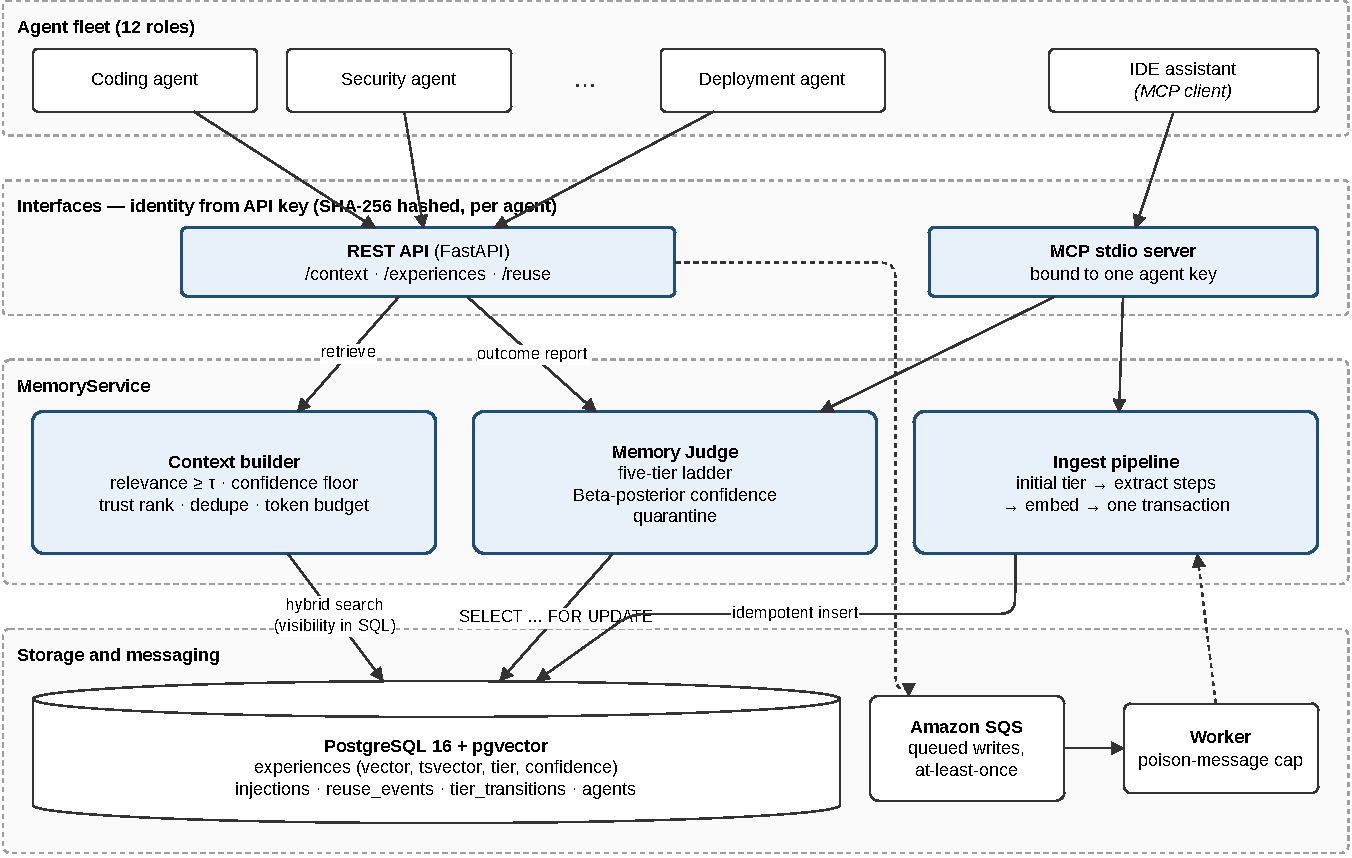
\includegraphics[width=0.86\textwidth]{figures/architecture.pdf}
\caption{\sysname{} architecture. Agents reach one \texttt{MemoryService} through a REST API or an MCP stdio server; identity always comes from an API key. Writes are processed in-request or through SQS by an idempotent worker; both paths run the same ingest pipeline.}
\label{fig:architecture}
\end{figure*}

\Cref{fig:architecture} shows the components. Agents use a REST API or the Model Context Protocol~\cite{mcp2024spec}; both call one \texttt{MemoryService}. Memories live in PostgreSQL with the pgvector extension~\cite{pgvector}. \Cref{fig:lifecycle} shows the four steps of an interaction: retrieve, act, store and report.

\subsection{Memory records and ingest}
\label{sec:ingest}
An experience is written by an ingest pipeline shared by the synchronous path and the queue worker. The pipeline (i) assigns an initial tier and confidence (\cref{sec:governance}); (ii) extracts a reusable procedure, either with an LLM that returns prerequisites, steps and pitfalls, or deterministically from numbered or \texttt{STEP:} lines; (iii) embeds the task text with its technology tags; and (iv) writes the row, the extracted procedure, the embedding and an audit record in a single transaction keyed by the experience identifier. Because the insert is idempotent, a redelivered queue message is a no-op, which makes at-least-once delivery safe.

We embed the task and its technology tags rather than the solution text. Queries at retrieval time are task descriptions, and including the long solution dilutes the similarity between two paraphrases of the same task.

\subsection{Retrieval and context selection}
\label{sec:retrieval}

\begin{figure*}[t]
\centering
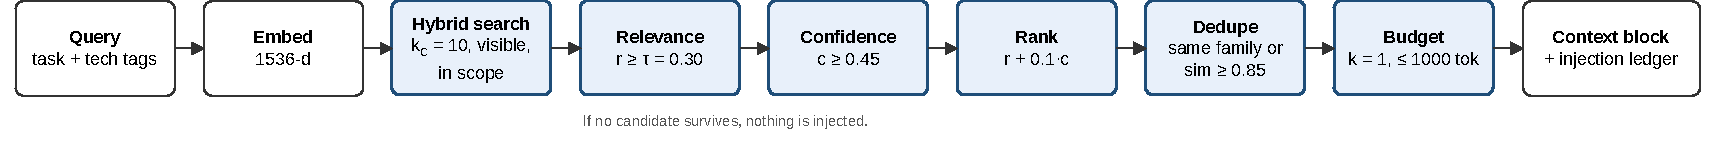
\includegraphics[width=\textwidth]{figures/pipeline.pdf}
\caption{Context selection. Each stage can only remove candidates; if none survive, nothing is injected.}
\label{fig:pipeline}
\end{figure*}

For a task $q$ with tags, \sysname{} retrieves the $k_c$ candidates that the requesting agent may see (\cref{sec:governance}), scored by
\begin{equation}
r(q,m) = \cos\!\big(e(q), e(m)\big) + \lambda\, \frac{\mathrm{rank}(q,m)}{1+\mathrm{rank}(q,m)},
\label{eq:relevance}
\end{equation}
where $e(\cdot)$ is the embedding, $\mathrm{rank}$ is PostgreSQL's full-text rank and $\lambda=0.15$. The second term is bounded in $[0,1)$, so $r$ stays on the cosine scale and can be thresholded. \Cref{alg:select} and \cref{fig:pipeline} give the selection. Two choices matter. First, when no candidate reaches the threshold $\tau$, nothing is injected; an irrelevant memory costs tokens and can mislead. Second, the default injection count is $k=1$; \cref{sec:ablations} shows why.

The default embedder is deterministic feature hashing~\cite{weinberger2009hashing} over word unigrams, bigrams and character 4-grams into 1536 signed dimensions. It runs offline and captures shared vocabulary, not paraphrase meaning; semantic embedding providers can be substituted without changing the rest of the system. $\tau$ is calibrated per embedder (\cref{sec:retrieval-results}).

\begin{algorithm}[t]
\caption{Context selection for agent $a$ and task $q$}
\label{alg:select}
\KwIn{task $q$, tags, agent $a$, policy $(k_c,\tau,c_{\min},\beta,\delta,k,B)$}
\KwOut{context block $C$, injected set $I$}
$\mathcal{M} \gets$ top-$k_c$ memories visible to $a$ by $r(q,\cdot)$\;
$\mathcal{M} \gets \{m \in \mathcal{M} : r(q,m) \ge \tau \wedge c(m) \ge c_{\min}\}$\;
sort $\mathcal{M}$ by $r(q,m) + \beta\, c(m)$, descending\;
$I \gets \emptyset$;\ $C \gets$ header\;
\ForEach{$m \in \mathcal{M}$}{
  \If{$\exists\, m' \in I$ : same family \textbf{or} $\mathrm{sim}(m,m') \ge \delta$}{\textbf{continue} \Comment*[r]{duplicate}}
  \lIf{$|I| = k$ \textbf{or} $|C \oplus \mathrm{fmt}(m)| > B$}{\textbf{break}}
  $C \gets C \oplus \mathrm{fmt}(m)$;\ $I \gets I \cup \{m\}$\;
}
record an injection $(m, a)$ for each $m \in I$\;
\Return $(C, I)$ \Comment*[r]{$C=\emptyset$ if $I=\emptyset$}
\end{algorithm}

The formatted block lists the task, prerequisites, numbered steps and known pitfalls, and marks memories recorded as failures so that they read as warnings. Averaged over all tasks, including those that receive nothing, the injected block costs 107 tokens (\cref{tab:main}).

\subsection{Governance}
\label{sec:governance}

\begin{figure*}[t]
\centering
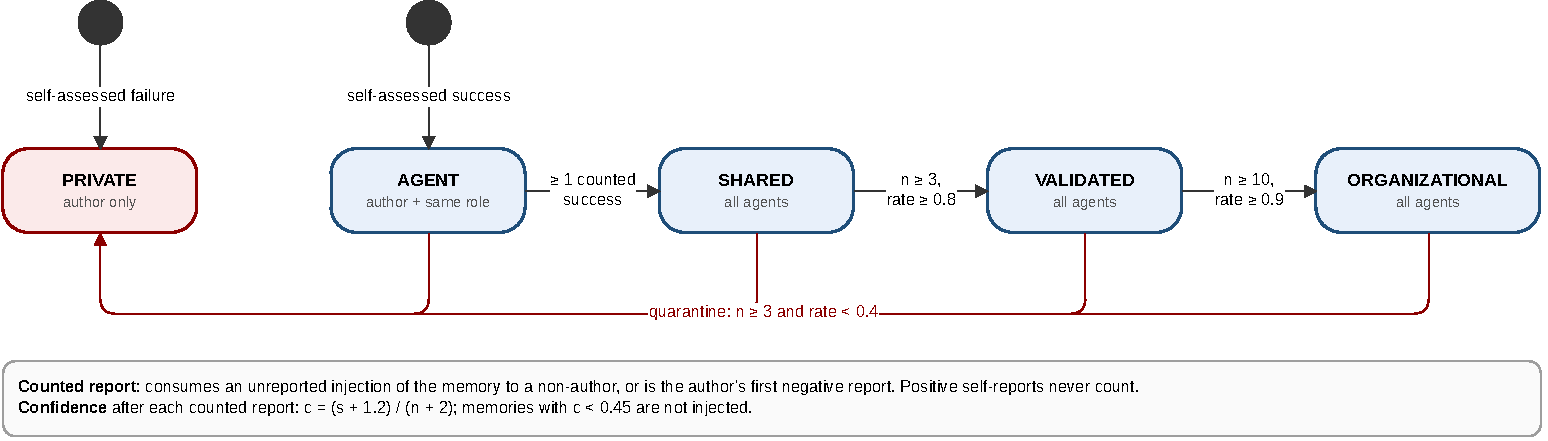
\includegraphics[width=0.95\textwidth]{figures/governance.pdf}
\caption{Memory Judge state machine. Visibility widens only on counted evidence from other agents; any tier can be quarantined.}
\label{fig:governance}
\end{figure*}

\paragraph{Tiers and visibility}
Each memory has a tier (\cref{fig:governance}). A memory the author judged successful enters at \textsc{agent}, visible to its author and to agents of the same role; a memory judged failed enters at \textsc{private}. Visibility is enforced inside the SQL query, not after it. Knowledge therefore spreads first within a role, where it is most likely to apply, and reaches the whole fleet only after other agents have used it successfully.

\paragraph{Counted reports}
After a task, an agent may report whether each injected memory worked. A report by agent $a$ on memory $m$ is \emph{counted} if and only if one of the following holds:
\begin{enumerate}
\item $a \neq \alpha(m)$ and there exists an injection $(m,a)$ that has not yet been reported; the report consumes it;
\item $a = \alpha(m)$, the report is negative, and $a$ has not previously made a counted negative report on $m$.
\end{enumerate}
All other reports are logged but ignored. Every counted report is applied under a row lock, together with the Judge's decision, in one transaction, so concurrent reports cannot act on stale counts.

\paragraph{Confidence}
Let $n$ and $s$ be the numbers of counted reports and counted successes. The confidence is the posterior mean of a Beta prior with mean $c_0=0.6$ and weight $w=2$~\cite{josang2002beta}:
\begin{equation}
c(m) = \frac{s + w\,c_0}{n + w}.
\label{eq:confidence}
\end{equation}
It is updated on every counted report. Memories with $c < c_{\min} = 0.45$ are not injected, so a new memory that fails once ($c=0.4$) stops spreading immediately, while one success raises it to $0.73$.

\paragraph{Promotion and quarantine}
\textsc{agent}$\to$\textsc{shared} after one counted success; \textsc{shared}$\to$\textsc{validated} at $n\ge3$ with rate $s/n\ge0.8$; \textsc{validated}$\to$\textsc{organizational} at $n\ge10$ with rate $\ge0.9$. Any memory with $n\ge3$ and rate $<0.4$ is quarantined to \textsc{private}. Every transition is recorded with its reason.

\paragraph{Author reputation (optional)}
Per-memory confidence cannot stop an author who writes a \emph{new} flawed memory for every task: each new memory starts from the global prior. With author reputation enabled, the prior of a new memory is instead its author's posterior over all counted reports on the author's earlier memories,
\begin{equation}
c_0(m) = \frac{S_{\alpha(m)} + w\,c_0}{N_{\alpha(m)} + w},
\label{eq:author}
\end{equation}
where $S_a$ and $N_a$ are the counted successes and reports on memories written by $a$, and \cref{eq:confidence} then uses $c_0(m)$ in place of $c_0$. An author whose memories keep failing starts every new memory below $c_{\min}$; an author without history starts at the global prior. The mechanism is off by default in the released configuration and is evaluated separately (\cref{sec:adversary}).

\begin{proposition}[Influence bound]
\label{prop:bound}
Let $S \subseteq \mathcal{A}$ be any set of agents and $m$ a memory with $\alpha(m) \notin S$. The number of counted successes that $S$ can add to $m$ is at most the number of injections of $m$ to members of $S$. If $\alpha(m) \in S$, $S$ can add no more counted successes than it could without the author, and at most one counted failure through the author.
\end{proposition}
\begin{proof}
A counted success from $a \neq \alpha(m)$ requires, by rule 1, an unreported injection $(m,a)$, and consumes it; injections are only created by the selection step for the requesting, authenticated agent. The author's reports count only if negative (rule 2), at most once.
\end{proof}

The bound matters because injections are not under the reporter's control: they happen only when the selection step chooses $m$ for that agent's task. A single agent cannot promote a peer's memory by repeated reports, and an author cannot promote its own memory at all. Collusion is still possible: colluders who legitimately receive each other's memories can report them as successes. \Cref{sec:adversary} measures how far this goes.

\subsection{Identity}
\label{sec:identity}
Each agent is registered by an administrator with a fixed role and receives a 256-bit random API key, of which only a SHA-256 hash is stored. The REST API derives the caller's identity and role from the key; requests that name a different agent are rejected. This closes three attacks present in designs that accept self-asserted identity: reading another agent's private memories by naming it, promoting one's own memory by reporting under a second name, and bypassing the author rule. Records the caller may not see are answered with \emph{not found}, so their existence is not revealed. Because registration is an administrative action, Sybil identities~\cite{douceur2002sybil} require the administrator's cooperation. When configured with a key, the MCP server binds all tool calls to that key's identity.

\begin{figure}[t]
\centering
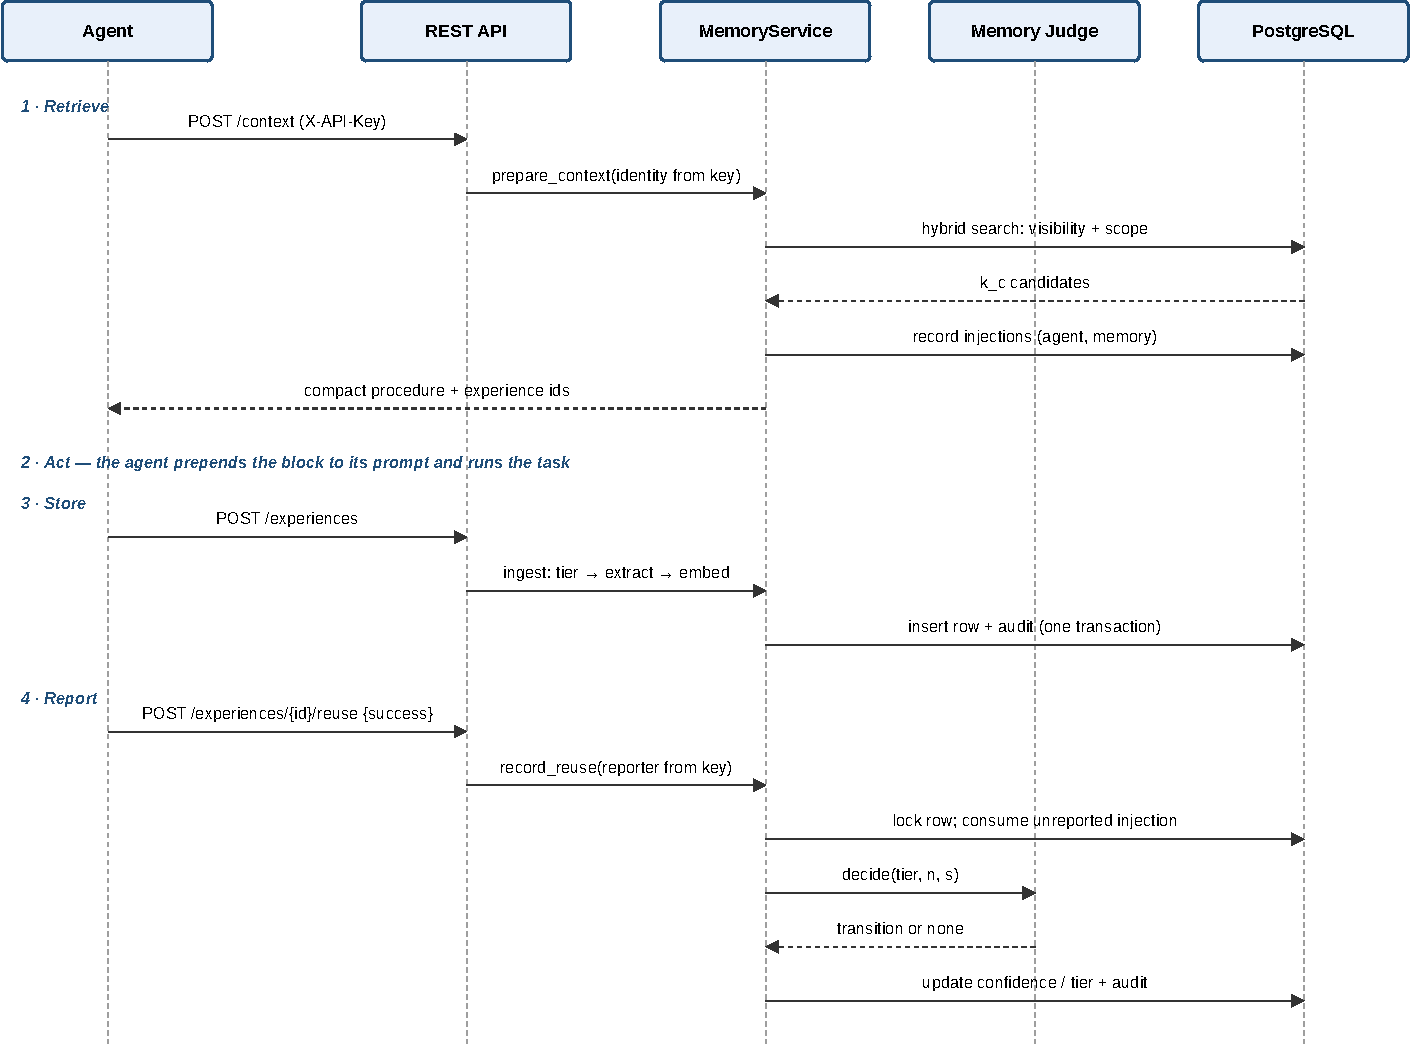
\includegraphics[width=\columnwidth]{figures/lifecycle.pdf}
\caption{One interaction. Injections are recorded at retrieval time; a later report is counted only against such a record.}
\label{fig:lifecycle}
\end{figure}

%% ===================================================================
\section{Implementation}
\label{sec:impl}

\sysname{} is written in Python (about 3,400 non-comment lines, plus 400 for the benchmark harness) on FastAPI, psycopg~3 and PostgreSQL~16 with pgvector. The schema has five tables: \texttt{experiences} (text, tags, procedure, embedding, tier, confidence, counters), \texttt{injections}, \texttt{reuse\_events}, \texttt{tier\_transitions} and \texttt{agents}. Visibility and run scoping are predicates in the retrieval query. Retrieval runs in one of two modes: \emph{exact}, which scores every visible memory, and \emph{index-backed}, in which an HNSW index~\cite{malkov2020hnsw} first selects the $N$ nearest memories by cosine and visibility, scope and the lexical term are applied to those only (\cref{sec:systems} compares them). Writes go either through Amazon SQS, with a worker that drops a message after a bounded number of failed deliveries, or directly through the same pipeline. The MCP server implements the 2024-11-05 protocol over stdio~\cite{mcp2024spec}. The system has 105 automated tests, including one test per attack in \cref{sec:identity} executed against the live API. Code, benchmark, experiment scripts and raw results are available in the repository (see \emph{Data availability}).

%% ===================================================================
\section{Evaluation methodology}
\label{sec:method}

\subsection{Benchmark}
The workload has 136 tasks in 45 families across all 12 roles (30 coding, 15 each for research, DevOps, testing and security, 10 deployment, and 6 each for documentation, data analysis, database, ML, cloud and monitoring). Tasks in a family are paraphrases, for example ``Implement exponential backoff retry decorator for boto3 SQS \texttt{receive\_message}'' and ``Add exponential backoff error recovery wrapper around SQS receive calls''. Each family has a ground-truth procedure of four steps, and each step has keyword checks that a correct answer must contain. We verified that no step's checks are satisfied by the text of the other steps, so the verifier detects any single missing step.

A \emph{strict} verdict requires all four steps and is the task's true outcome. A \emph{lenient} verdict allows one missing step and models the agent's own self-assessment: it is what the agent stores as success. Some stored successes are therefore flawed, which is the realistic failure mode governance must handle.

\subsection{Simulated agent environment}
\label{sec:sim}
Task outcomes come from a simulated agent that implements the LLM interface. It parses the injected context back into memories and decides as follows; all parameters are listed in \cref{tab:sim}.
\begin{itemize}
\item With an applicable memory from the task's own family that contains the full procedure, it follows the memory: a short answer, succeeding unless it slips.
\item With an applicable but incomplete memory, it is misled with probability $p_{\mathrm{mislead}}$ and reproduces the gap; otherwise it solves from scratch.
\item Otherwise it solves from scratch: a long answer with the full procedure with probability $p_{\mathrm{solve}}$, and one or two missing steps otherwise. Irrelevant injected memories reduce $p_{\mathrm{solve}}$ by $p_{\mathrm{distract}}$.
\end{itemize}
Memories marked as failures are treated as warnings and never followed. All randomness is seeded per task instance, so every arm sees the same luck on the same task (common random numbers). Input tokens are counted from the actual prompt, including the injected block; output tokens and latency follow the parameters.

\begin{table}[t]
\centering
\caption{Simulated agent parameters. The benefit of a correct memory is an assumption encoded here; \cref{sec:sensitivity} varies the two most consequential ones.}
\label{tab:sim}
\small
\setlength{\tabcolsep}{4pt}
\begin{tabular}{@{}lr@{}}
\toprule
Parameter & Value \\
\midrule
$p_{\mathrm{solve}}$: success, no applicable memory & 0.65 \\
\quad on failure, one step missing (else two) & 0.60 \\
$p_{\mathrm{slip}}$: failure following a correct memory & 0.03 \\
$p_{\mathrm{mislead}}$: follow an incomplete memory & 0.85 \\
$p_{\mathrm{distract}}$: penalty, irrelevant context & 0.05 \\
Output tokens, from scratch & $690 + U[0,300)$ \\
Output tokens, following a memory & $250 + U[0,60)$ \\
Latency (ms) & $300 + 8 \times$ output \\
Price, USD / $10^6$ tokens (in / out) & 3 / 15 \\
\bottomrule
\end{tabular}
\end{table}

\subsection{Arms, protocol and metrics}
We compare three arms: \emph{no memory}; \emph{flat shared memory}, in which every experience is visible to every agent immediately and no outcome feedback is used; and \sysname{} with $k=1$, $\tau=0.30$, $c_{\min}=0.45$ and feedback probability $\phi=0.7$. Each arm runs the 136 tasks for three epochs (408 task instances) in a shuffled order that is identical across arms, with three agents per role, for five seeds. Every arm has its own run identifier and retrieval is scoped to it, so no arm can read another's memories.

\emph{Task success} is the strict verdict. \emph{Retrieval precision} is the share of injected memories from the task's own family. \emph{Flawed injections} is the share of same-family injections whose memory came from a task that actually failed. \emph{Misled rate} is the share of tasks that received a same-family memory and still failed. The \emph{redundancy index} is the share of tasks whose family had already been solved in the run but that were solved again without a same-family memory. We report mean and standard deviation over seeds, exact McNemar tests on the $5\times408$ paired task instances, and bootstrap confidence intervals for per-task token savings.

%% ===================================================================
\section{Results}
\label{sec:results}

\subsection{Main comparison}
\label{sec:main}

\begin{table*}[t]
\centering
\caption{Main results (mean $\pm$ s.d. over five seeds, 408 task instances per seed). Task success is the strict, verified outcome.}
\label{tab:main}
\small
\begin{tabular}{@{}lrrrrrrr@{}}
\toprule
Arm & Success (\%) & Precision (\%) & Flawed inj.\ (\%) & Misled (\%) & Redund.\ index & Tokens/task & Ctx tokens \\
\midrule
No memory & $65.0 \pm 2.9$ & -- & -- & -- & $1.000$ & $928 \pm 4$ & 0 \\
Flat shared memory & $75.4 \pm 4.9$ & $95.2 \pm 0.3$ & $27.7 \pm 5.3$ & $22.5 \pm 5.1$ & $0.017$ & $608 \pm 14$ & $112 \pm 1$ \\
\sysname{} & $\mathbf{86.8 \pm 1.1}$ & $95.0 \pm 1.1$ & $\mathbf{4.4 \pm 1.0}$ & $\mathbf{7.1 \pm 1.2}$ & $0.029$ & $\mathbf{591 \pm 5}$ & $\mathbf{107 \pm 2}$ \\
\bottomrule
\end{tabular}
\end{table*}

\begin{figure*}[t]
\centering
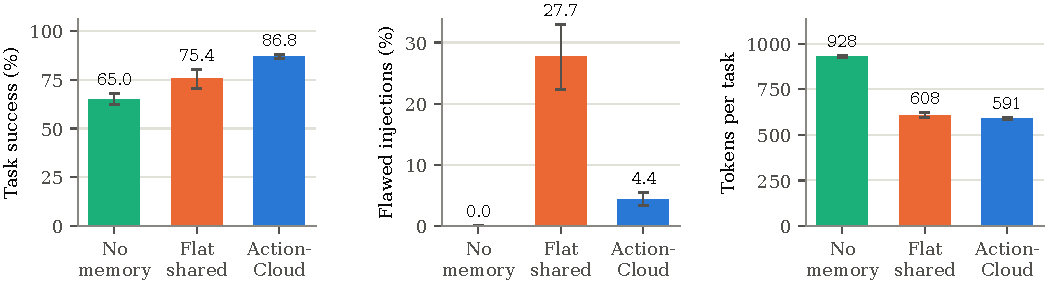
\includegraphics[width=\textwidth]{figures/main_results.pdf}
\caption{Main comparison. Error bars: s.d. over five seeds.}
\label{fig:main}
\end{figure*}

\Cref{tab:main} and \cref{fig:main} summarise the three arms. Both memory arms retrieve the right family about 95\% of the time and almost never re-derive a solved family (redundancy index below 0.03). They differ in \emph{what} they inject. In the flat memory, 27.7\% of same-family injections carry a flawed procedure; with \sysname{} the rate is 4.4\%. The misled rate falls from 22.5\% to 7.1\% and task success rises from 75.4\% to 86.8\%. Governance also makes the outcome more stable: the standard deviation of success across seeds drops from 4.9 to 1.1 points, because a flawed memory that happens to be stored early no longer dominates its family for the rest of the run.

On the $2{,}040$ paired task instances, \sysname{} succeeded where flat memory failed 252 times and the reverse happened 21 times (exact McNemar $p = 1.8\times10^{-51}$); against no memory the counts are 523 and 78 ($p = 7.6\times10^{-82}$). Per-task token use falls by 36.0\% relative to no memory (95\% bootstrap CI 35.1--36.9\%). These tests quantify effects \emph{within} the simulated environment and should be read with \cref{sec:sensitivity}.

\begin{figure}[t]
\centering
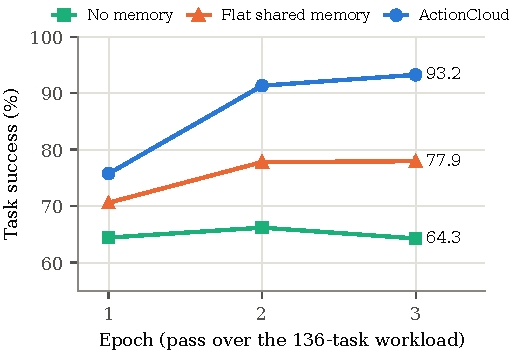
\includegraphics[width=\columnwidth]{figures/learning_curve.pdf}
\caption{Success by epoch, averaged over five seeds. The first epoch contains the first encounter with most families.}
\label{fig:learning}
\end{figure}

\Cref{fig:learning} shows how the gap develops. In the first epoch most families are new, and both memory arms are only somewhat better than no memory (70.6\% and 75.7\% against 64.4\%). In later epochs \sysname{} reaches 91.3\% and 93.2\%, while flat memory stalls near 78\%: its flawed memories keep being retrieved and copied. The final tier distribution of one representative seed illustrates the mechanism: of 408 memories, 299 remained at \textsc{agent}, 83 were promoted to \textsc{shared}, 10 to \textsc{validated}, and 16 were \textsc{private}. The gain over no memory is positive for every role, from $+15.5$ points (monitoring) to $+31.1$ (cloud and DevOps); the six-task roles contribute only 18 instances per seed, so per-role differences are noisy.

\subsection{Retrieval quality}
\label{sec:retrieval-results}

\begin{figure*}[t]
\centering
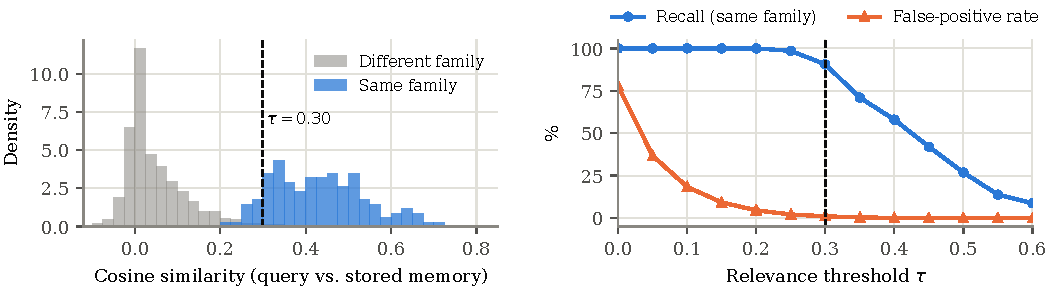
\includegraphics[width=\textwidth]{figures/calibration.pdf}
\caption{Retrieval calibration on all ordered task pairs. Left: cosine similarity for pairs from the same family and from different families. Right: recall and false-positive rate against the threshold $\tau$; dashed line: the default $\tau=0.30$.}
\label{fig:calibration}
\end{figure*}

\Cref{fig:calibration} shows similarity distributions over all $136\times135$ ordered task pairs. At $\tau=0.30$, 90.6\% of same-family pairs clear the threshold and 1.0\% of different-family pairs do. The nearest stored neighbour of a task belongs to its family for 128 of 136 tasks (94.1\%). This figure depends strongly on including the technology tags in the query: with the task text alone it falls to 75 of 136 (55.1\%). Tasks in one family share their tags in this benchmark, which favours a lexical embedder; paraphrases with no shared vocabulary require a semantic embedder, and $\tau$ must be recalibrated for it.

\subsection{Ablations}
\label{sec:ablations}

\begin{figure*}[t]
\centering
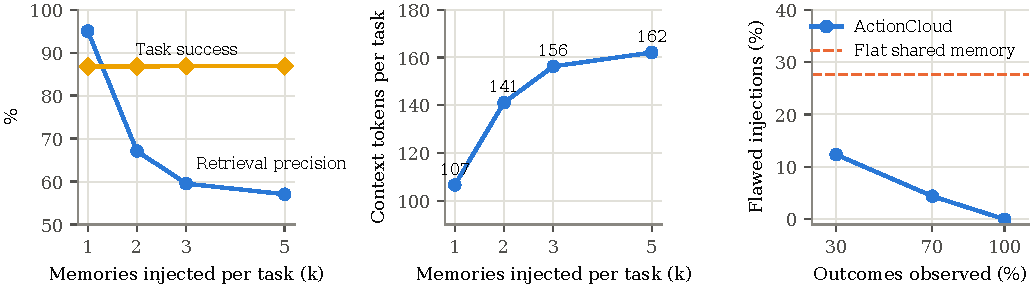
\includegraphics[width=\textwidth]{figures/ablations.pdf}
\caption{Ablations (five seeds). Left, centre: effect of the number of injected memories $k$. Right: flawed injections against the share of task outcomes observed; dashed: flat shared memory.}
\label{fig:ablations}
\end{figure*}

\paragraph{How many memories to inject}
Increasing $k$ from 1 to 5 lowers retrieval precision from 95.0\% to 57.0\% and raises context from 107 to 162 tokens per task, while success does not change (86.8--86.9\% at every $k$) (\cref{fig:ablations}). The additional memories come from other families: once the redundancy filter has kept one memory per family, the next candidates are less relevant. Token savings against no memory fall from 36.4\% to 30.9\%. One well-chosen memory is the better operating point.

\paragraph{Relevance threshold}
With $\tau=0$ the top candidate is always injected. Injection rate rises from 84.4\% to 97.7\%, precision falls to 79.9\%, and success falls by 2.5 points to 84.3\%.

\paragraph{Observability of outcomes}
Governance acts on observed outcomes, so its value depends on $\phi$. When 30\%, 70\% and 100\% of outcomes are observed, flawed injections are 12.3\%, 4.4\% and 0.0\%, and success is 81.5\%, 86.8\% and 89.8\%, against 27.7\% and 75.4\% for flat memory. Even sparse feedback helps, but a deployment in which outcomes are rarely observable would gain little from governance.

\subsection{Adversarial agents}
\label{sec:adversary}

\begin{figure*}[t]
\centering
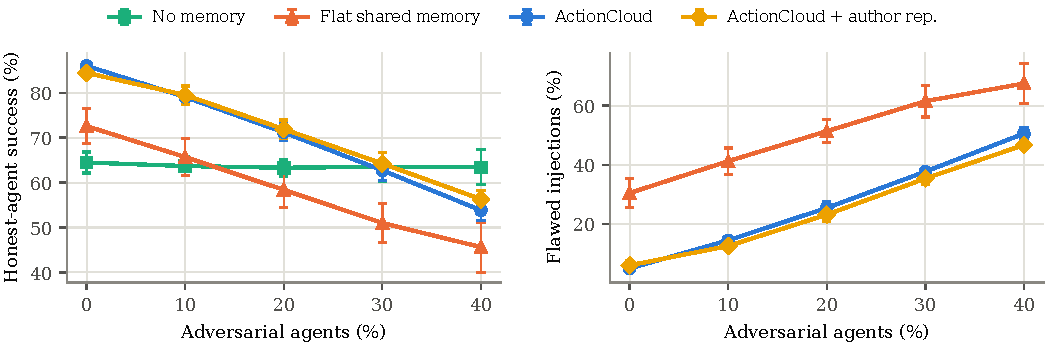
\includegraphics[width=\textwidth]{figures/adversary.pdf}
\caption{Robustness to adversarial agents that store flawed procedures as successes, report every received memory as a success, never report their own failures and thereby collude. Success is measured over honest agents only (ten agents per role, three seeds; error bars: s.d.).}
\label{fig:adversary}
\end{figure*}

We now make a share of the agents adversarial in the sense of \cref{sec:problem}: each stores a procedure missing two steps, labelled as a success, for every task it performs; reports every memory it receives as a success, including those of other adversaries; and never reports its own memories as failed. We use ten agents per role so that shares of 10--40\% are exact, and measure success over honest agents only (\cref{fig:adversary}).

Governance always beats the flat memory, which degrades fastest: its honest-agent success falls from 72.6\% to 45.6\% as the adversary share grows from 0 to 40\%, well below the 63--64\% of agents without memory. \sysname{} degrades more slowly (from 86.0\% to 53.8\%) and cuts flawed injections by 17 to 27 points at every share. It does not, however, contain a large coalition. At 20\% adversaries it still improves on no memory by 7.9 points; at 30\% it is level with no memory (62.7\% against 63.5\%); at 40\% it is 9.6 points worse. Two properties of the attack explain this. Each adversary writes a \emph{new} flawed memory for every task, so per-memory evidence never accumulates against it; and colluders that legitimately receive each other's memories produce counted successes, which \cref{prop:bound} permits.

Author reputation (\cref{eq:author}) targets the first property. It lowers flawed injections by 1.9 to 3.9 points at adversary shares of 10--40\% and raises honest-agent success by up to 2.5 points at 40\%, but it does not move the break-even point, and it has a cost when all agents are honest: over five benign seeds, success falls from 86.8\% ($\pm1.1$) to 83.4\% ($\pm2.8$), because honest authors whose early memories failed through bad luck start later memories below the confidence floor. We therefore leave it disabled by default. Outcome evidence alone cannot defeat collusion at this scale; weighting reports by the reporter's own credibility, or requiring reports from agents outside the author's coalition, is necessary and left to future work.

\subsection{Sensitivity to the simulator's assumptions}
\label{sec:sensitivity}

\begin{figure*}[t]
\centering
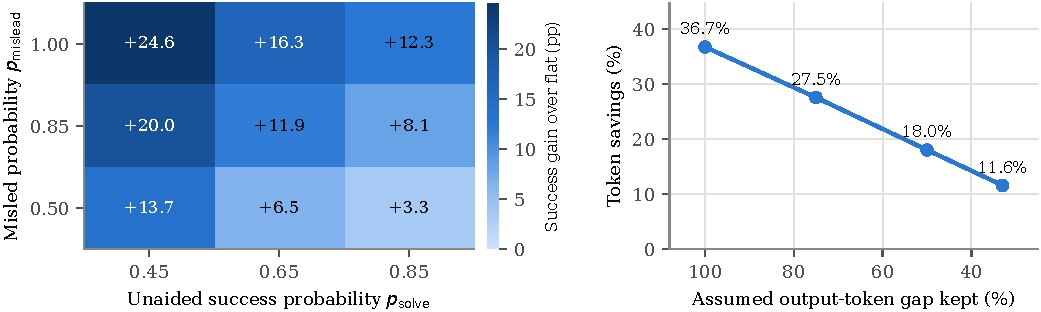
\includegraphics[width=\textwidth]{figures/sensitivity.pdf}
\caption{Sensitivity analysis (two seeds per cell). Left: success gain of \sysname{} over the flat memory across the two behavioural parameters that most affect the comparison. Right: token savings over no memory when the assumed gap in output tokens between solving from scratch and following a memory is shrunk.}
\label{fig:sensitivity}
\end{figure*}

\Cref{fig:sensitivity} varies the two parameters that most affect the comparison between memory arms, the unaided success probability $p_{\mathrm{solve}}\in\{0.45,0.65,0.85\}$ and the probability of being misled by an incomplete memory $p_{\mathrm{mislead}}\in\{0.5,0.85,1.0\}$. \sysname{} beats the flat memory in all nine settings, by 3.3 to 24.6 points, and beats no memory in all nine, by 6.3 to 31.2 points. The gain over flat memory is largest when agents are weak and easily misled, because flawed memories are then both more common and more harmful. The flat memory, in contrast, is \emph{worse} than no memory in two settings with competent agents ($p_{\mathrm{solve}}=0.85$ with $p_{\mathrm{mislead}}\ge0.85$). Across the grid, \sysname{} keeps flawed injections between 2.9\% and 9.0\%, against 13.4\% to 51.9\% for the flat memory. The qualitative conclusion, that governance matters more than retrieval once memory is shared, holds throughout the range we tested.

Token savings do not. They follow almost entirely from the assumed difference in output length between solving from scratch and following a procedure. When that difference is reduced to 75\%, 50\% and 33\% of its default, savings fall from 36.7\% to 27.5\%, 18.0\% and 11.6\%. The input cost of the injected block is small by comparison, but the size of the saving on a real model is an open empirical question.

\subsection{Systems performance}
\label{sec:systems}

\begin{table}[t]
\centering
\caption{Measured service latency (PostgreSQL~16 with pgvector~0.6 and the service on one 2-vCPU Intel Xeon 2.8\,GHz virtual machine; hashing embedder).}
\label{tab:systems}
\small
\setlength{\tabcolsep}{4pt}
\begin{tabular}{@{}lrr@{}}
\toprule
Operation & p50 (ms) & p95 (ms) \\
\midrule
Ingest (tier, extract, embed, transactional insert) & 11.3 & 16.0 \\
Outcome report (lock, injection, Judge, audit) & 4.6 & 8.4 \\
Embedding a query (hashing, 1536-d) & \multicolumn{2}{c}{0.6 (mean)} \\
\midrule
Context build, 1k memories, exact & 51 & 62 \\
Context build, 50k memories, exact & 1254 & 1597 \\
Context build, 50k memories, HNSW ($N{=}200$) & 17 & 24 \\
\bottomrule
\end{tabular}
\end{table}

\begin{figure}[t]
\centering
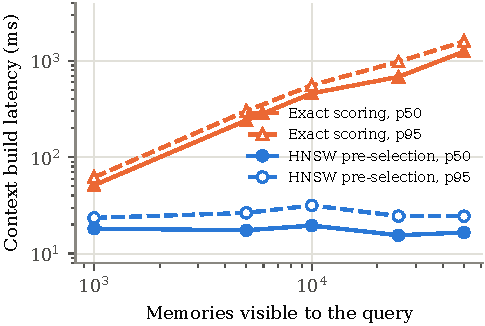
\includegraphics[width=\columnwidth]{figures/scaling.pdf}
\caption{Context-build latency against the number of memories visible to the query (60 queries per point). HNSW pre-selection chose the same injected memory as exact scoring for every query at every size.}
\label{fig:scaling}
\end{figure}

\Cref{tab:systems} and \cref{fig:scaling} report latencies measured on the service itself, not in simulation. Ingesting an experience takes 11.3\,ms at the median, about 90 per second on one connection, and applying an outcome report, including the row lock, injection lookup, Judge decision and audit rows, takes 4.6\,ms. Both are small next to an LLM call.

Retrieval is where scale matters. Exact scoring evaluates the similarity and full-text rank of every visible memory, so its latency grows roughly linearly, from 51\,ms with 1,000 visible memories to 461\,ms at 10,000 and 1.25\,s at 50,000. With HNSW pre-selection of the 200 nearest memories, the context build takes 15--20\,ms at every size we measured, and it injected the same memory as exact scoring in all 300 measured queries. We use exact scoring in the evaluation because it is deterministic and the per-run stores are small; deployments beyond a few thousand memories should use the index-backed mode. Because pgvector~0.6 applies filters after the index scan, the candidate count $N$ must exceed the number of invisible memories among the true neighbours; in stores dominated by other agents' private memories, $N$ must grow accordingly.


%% ===================================================================
\section{Discussion}
\label{sec:discussion}

\paragraph{What the evidence establishes}
Three results depend only on quantities \sysname{} controls or measures directly: retrieval calibration (\cref{fig:calibration}), which memories are injected and how often they are flawed, and the cost of the service itself (\cref{sec:systems}). Under the stated assumptions, and across the ranges in \cref{sec:sensitivity}, governance sharply reduces the injection of flawed procedures relative to an ungoverned shared memory, and a single injected memory dominates several.

\paragraph{What it assumes}
How much an agent gains from a correct memory, and how easily it is misled by a flawed one, are parameters of the simulated agent, not measurements. The absolute success rates, the size of the success gain and the token savings all depend on them. They should not be quoted as properties of any LLM. The experiment that would settle them runs the same harness with a real model; the harness supports it without changes to the verifier or metrics.

\paragraph{Threats to validity}
\emph{Internal}: the simulated agent treats memories marked as failures as warnings and never follows them; a real model may not. \emph{Construct}: the verifier checks for required steps by keyword and would accept an answer that mentions a step without performing it. \emph{External}: the benchmark is synthetic, families share technology tags, and cross-role reuse is rare because most families belong to one role. \emph{Configuration}: the promotion thresholds and confidence prior were set by design rather than tuned; we did not search for values that favour \sysname{}. \emph{Baselines}: we compare against no memory and an ungoverned shared memory built on the same retrieval, which isolates the effect of governance but is not a comparison with other memory systems; systems such as Mem0~\cite{chhikara2025mem0} or MemClaw~\cite{margalit2026governed} target different settings and interfaces, and a head-to-head evaluation on a common fleet benchmark remains to be done.

\paragraph{Deployment implications}
Governance needs observable outcomes. Deployments where agents run tests, receive CI results or see a deployment succeed provide them naturally; purely conversational agents may not. The confidence floor, not formal quarantine, did most of the work in our runs: a flawed memory usually stopped being injected after its first failed reuse, long before it accumulated the three reports needed for quarantine.

%% ===================================================================
\section{Limitations and future work}
\label{sec:limitations}
The central limitation is the absence of a real-LLM evaluation; it is the next experiment. Semantic embeddings are implemented but not evaluated. Index-backed retrieval agreed with exact retrieval in all our measurements, but with pgvector~0.6 it filters after the index scan and can miss visible memories when invisible ones crowd the neighbourhood; filtered index scans in newer pgvector versions would remove this caveat. API keys do not expire and requests are not rate-limited. Colluding adversaries can still promote each other's memories within the influence bound, and we have not studied adaptive adversaries that behave honestly until trusted. Finally, promotion is per memory; supersession of outdated procedures and cross-family generalisation are left open.

%% ===================================================================
\section{Conclusion}
\label{sec:conclusion}
Sharing experience across a fleet of LLM agents saves work only if the fleet does not also share its mistakes. \sysname{} treats trust in a stored procedure as earned from authenticated outcome reports that are tied to actual injections, and injects a single compact procedure per task. In a controlled environment with explicit assumptions, this reduced the injection of flawed procedures by a factor of six relative to an ungoverned shared memory, with a per-request overhead of a few milliseconds for writes and reports and about 17\,ms for retrieval over 50,000 memories with the approximate index. The code, benchmark and results are released so that the remaining question, how much real models gain, can be answered with the same instruments.

%% ===================================================================
\section*{CRediT authorship contribution statement}
\textbf{[Author 1]}: Conceptualization, Software, Writing -- original draft. \textbf{[Author 2]}: [roles]. \textbf{[Author 3]}: [roles]. \textbf{[Author 4]}: [roles]. \textbf{[Author 5]}: [roles].

\section*{Declaration of competing interest}
The authors declare that they have no known competing financial interests or personal relationships that could have appeared to influence the work reported in this paper.

\section*{Data availability}
The source code, benchmark, experiment scripts and raw results are available at \url{https://github.com/nagashiva23/action-cloud}.

\section*{Declaration of generative AI and AI-assisted technologies in the manuscript preparation process}
During the preparation of this work the authors used [name of tool / service] in order to [reason]. After using this tool/service, the authors reviewed and edited the content as needed and take full responsibility for the content of the published article.

\bibliographystyle{elsarticle-num}
\bibliography{refs}

\end{document}
